\documentclass{HSP-Experiment} % Options available : code, tikz-cross
\usepackage[utf8]{inputenc}
\usepackage[french]{babel}
\usepackage{wrapfig}

% Settings :
%\definecolor{cPrim}{gray}{0.37}
\colorlet{cPrim}{Blue}

\title{Experiment n°? : ???}
\class{CLASS}
\date{Semaine n°15}

\graphicspath{{Figures/}}

%%%%%%%%%%%%%%%%%%%%%%%%%%%%% Custom commands %%%%%%%%%%%%%%%%%%%%%%%%%%%%%%
\usetikzlibrary{calc}
\newcommand{\lines}[1]{
	\newline
	\begin{tikzpicture}
	\foreach \number in {1,...,#1}{
		\draw[] (0, \number*2em) -- (\linewidth, \number*2em);
	}
	\draw[white!0] (0, #1*2em)+(0,2em) -- ($(0, #1*2em)+(0,2em)$);
	\end{tikzpicture}
}
%%%%%%%%%%%%%%%%%%%%%%%%%%%%%%%%%%%%%%%%%%%%%%%%%%%%%%%%%%%%%%%%%%%%%%%%%%%%

\begin{document}
	\maketitle
	
	Un crayon semble se briser lorsqu'il entre dans l'eau. Il s'agit simplement d'une illusion d'optique due au phénomène de \textbf{réfraction}.\\
	
	\textbf{Objectif de l'activité :} Quelle relation mathématique illustre le phénomène de réfraction ?
	
	\begin{doc}[Découverte de la loi de la réfraction]
		\vspace*{-\baselineskip}
		\begin{multicols}{2}
			\begin{itemize}
				\item La \textbf{normale} est la droite perpendiculaire à la surface de séparation de deux milieux transparents et passant par le point d'incidence I.
				\item Les angles d'\textbf{incidence} ($i_1$) et de \textbf{réfraction} ($i_2$) sont mesurés par rapport à la normale.
				\item W.S\textsc{nell} (1580 -- 1626) et R.D\textsc{escartes} (1596 -- 1650) montrent qu'il y a proportionnalité entre le sinus de l'angle d'incidence ($i_1$) et le sinus de l'angle de réfraction ($i_2$), énoncé ainsi :
				$$\sin(i_1) = k \times \sin(i_2)$$
				où $k$ est une constante.
			\end{itemize}
		
			\begin{center}
				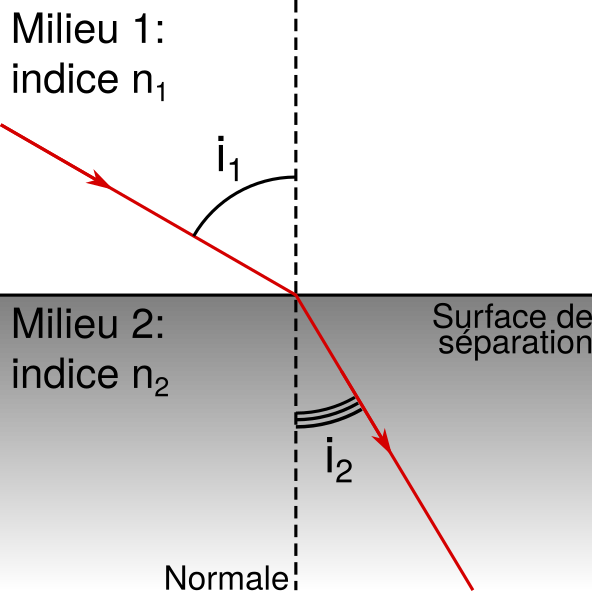
\includegraphics[scale=1]{SD}
			\end{center}
		\end{multicols}
	\end{doc}
	
	\begin{doc}[Matériel]
		\begin{itemize}
			\item Disque gradué
			\item Lanterne simulant un rayon lumineux
			\item Demi-cylindre de plexiglas
		\end{itemize}
	\end{doc}
	
	\begin{enumerate}
		\item Utiliser le dispositif expérimental pour mesurer les angles de réfraction $i_2$ en fonction des angles d'incidence $i_1$. Écrire les résultats dans le tableau suivant.
	\end{enumerate}
	
	\begin{center}
		\renewcommand{\arraystretch}{1.5}
		\resizebox{\linewidth}{!}{
		\begin{tabular}{|>{\columncolor{cPrim!25}\centering}m{2cm}
						|>{\centering}m{1.5cm}
						|>{\centering}m{1.5cm}
						|>{\centering}m{1.5cm}
						|>{\centering}m{1.5cm}
						|>{\centering}m{1.5cm}
						|>{\centering}m{1.5cm}
						|>{\centering}m{1.5cm}
						|>{\centering\arraybackslash}m{1.5cm}|
					   }
			\hline
			\textbf{Angle d'incidence $\mathbf{i_1}$ (°)}   & 0 & 10 & 20 & 30 & 40 & 50 & 60 & 70 \\ \hline
			\textbf{Angle de réfraction $\mathbf{i_2}$ (°)} &   &    &    &    &    &    &    &    \\ \hline
			$\mathbf{sin(i_1)}$                     & \vspace{1cm}\null  &    &    &    &    &    &    &    \\ \hline
			$\mathbf{sin(i_2)}$                     & \vspace{1cm}\null  &    &    &    &    &    &    &    \\ \hline
		\end{tabular}}
	\end{center}
	
	\begin{enumerate}[resume]
		\item À l'aide de la calculatrice paramétrée en degré, compléter le tableau avec les valeurs du sinus de $i_1$ ($\sin i_1$) du sinus de $i_2$ ($\sin i_2$).\\
		
		\item Vérifier qu'il y a proportionnalité entre $\sin i_1$ et $\sin i_2$ comme l'ont énoncé W.S\textsc{nell} et R.D\textsc{escartes}.
		\lines{4}
		% On voit que l'on passe d'une ligne à l'autre en multipliant par le même chiffre : k= ??? (1.5 ou 1.33)
		
		\item On sait aujourd'hui que le coefficient $k$ peut s'écrire comme le rapport de deux grandeurs :
		$$k = \frac{n_2}{n_1}$$
	\end{enumerate}

	\begin{ToRemember}{Loi de Snell-Descartes}
		\hspace{0.8\parindent} Comment peut-on réécrire la \textbf{loi de Snell-Descartes} ? \vspace{10\baselineskip}
	\end{ToRemember}
\end{document}